%% LaTeX Beamer presentation template (requires beamer package)
%% see http://latex-beamer.sourceforge.net/
%% idea contributed by H. Turgut Uyar
%% template based on a template by Till Tantau
%% this template is still evolving - it might differ in future releases!

\documentclass{beamer}
\usepackage[brazil]{babel}
\usepackage[utf8]{inputenc}
\usepackage{amsfonts}
\usepackage{amsmath}
\usepackage{float}
\usepackage{subfig}

\mode<presentation>
{
    \usetheme{PaloAlto}
    
    \setbeamercovered{transparent}
}


\title{Sistema TRUE}
%\subtitle{}

% - Use the \inst{?} command only if the authors have different
%   affiliation.
\author{Danilo Ávila e Tales Porto}
%\author{\inst{1}}

% - Use the \inst command only if there are several affiliations.
% - Keep it simple, no one is interested in your street address.
\institute[UnB]
{
    %\inst{1}%
    Departamento de Ciência da Computação\\
    Instituto de Ciências Exatas\\
    Universidade de Brasília
}

\date{07 de dezembro de 2011}


% This is only inserted into the PDF information catalog. Can be left
% out.
%\subject{Talks}



% If you have a file called "university-logo-filename.xxx", where xxx
% is a graphic format that can be processed by latex or pdflatex,
% resp., then you can add a logo as follows:

% \pgfdeclareimage[height=0.5cm]{university-logo}{university-logo-filename}
% \logo{\pgfuseimage{university-logo}}



% Delete this, if you do not want the table of contents to pop up at
% the beginning of each subsection:
%\AtBeginSubsection[]
%{
%\begin{frame}<beamer>
%    \frametitle{Sumário}
%    \tableofcontents[currentsection,currentsubsection]
%    \end{frame}
%}

% If you wish to uncover everything in a step-wise fashion, uncomment
% the following command:

%\beamerdefaultoverlayspecification{<+->}

\begin{document}

% ------------- TITLE PAGE -------------
\begin{frame}
\titlepage
\end{frame}
% ------------- TITLE PAGE -------------


% ------------- SUMARIO -------------
\begin{frame}
	\frametitle{Sumário}
	\tableofcontents
\end{frame}


% ------------- Introdução -------------
\section{Introdução}

	\subsection{Computação Ubíqua}
		\begin{frame}
	    	\frametitle{Computação Ubíqua}
		\end{frame}
		
	\subsection{SmartSpace}
		\begin{frame}
	    	\frametitle{SmartSpace}
		\end{frame}
		
	\subsection{UnBquitous}
		\begin{frame}
	    	\frametitle{UnBquitous}
		\end{frame}

% ------------- Problema -------------
\section{Problema}

	\begin{frame}
    	\frametitle{Problema}
    	Qual a melhor forma do middleware conhecer a identidade dos usuários
    	presentes no SmartSpace?
	\end{frame}

% ------------- Hipoteses e objetivos -------------
\section{Hipóteses e objetivos}

	\begin{frame}
    	\frametitle{Hipóteses e objetivos}
    	Acreditando em um sensor, relativamente novo, denomidado \textif{Kinect} e
    	na confiabilidade do \textit{Eigenfaces}, algoritmo de reconhecimento
    	facial, objetivamos desenvolver um sistema que rastreasse e reconhecesse os
    	usuários presentes no SmartSpace provendo ao middleware informações de
    	identificação e localização. A esse sistema foi dado o nome de TRUE.
	\end{frame}
	
% ------------- Sistema TRUE -------------
\section{Sistema TRUE}

	\begin{frame}
    	\frametitle{Sistema TRUE}
    	
    	TRUE \rightarrow \textit{\textbf{T}racking and \textbf{R}ecognizing
    	\textbf{U}sers in the \textbf{E}nvironment}.
    	
    	O sistema TRUE se divide em 4 modulos:
    		\begin{itemize}
    		  \item \textbf{Rastreamento}
    		  \item \textbf{Reconhecimento}
    		  \item \textbf{Registro}
    		  \item \textbf{Integração}
    		\end{itemize}
    \end{frame}
    
	% ------------- Sistema TRUE -> Rastreamento -------------
    \subsection{Rastreamento}
		\begin{frame}
	    	\frametitle{Sistema TRUE - Rastreamento}
	    	
	    \end{frame}
    
	% ------------- Sistema TRUE -> Reconhecimento -------------
    \subsection{Reconhecimento}
		\begin{frame}
	    	\frametitle{Sistema TRUE - Reconhecimento}
	    	
	    \end{frame}
    
	% ------------- Sistema TRUE -> Registro -------------
    \subsection{Registro}
		\begin{frame}
	    	\frametitle{Sistema TRUE - Registro}
	    	
	    \end{frame}
    
	% ------------- Sistema TRUE -> Integração -------------
    \subsection{Integração}
		\begin{frame}
	    	\frametitle{Sistema TRUE - Integração}
	    	
	    \end{frame}
    
	% ------------- Sistema TRUE -> Relação entre os modulos -------------
    \subsection{Relação entre os modulos}
		\begin{frame}
	    	\frametitle{Sistema TRUE - Relação entre os modulos}
	    	
	    \end{frame}

% ------------- Resultados obtidos -------------
\section{Resultados obtidos}

   	\begin{frame}
    	\frametitle{Resultados obtidos}
    \end{frame}

	% ------------- Resultados obtidos -> Rastreamento -------------
    \subsection{Rastreamento}
    	\begin{frame}
	    	\frametitle{Rastreamento - Detecção}
	    	
			\begin{figure}[htb]
				\begin{center}
					\subfloat[] {
						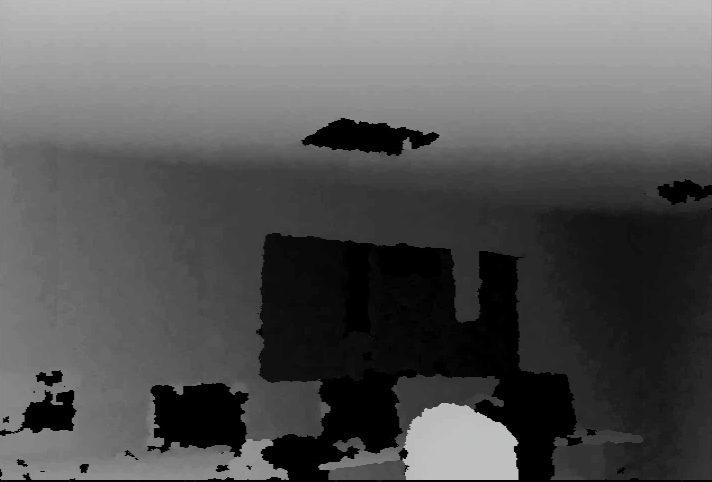
\includegraphics[width=0.24\textwidth]{figuras/5.Testes/deteccao/1.png}}
					\subfloat[] {
						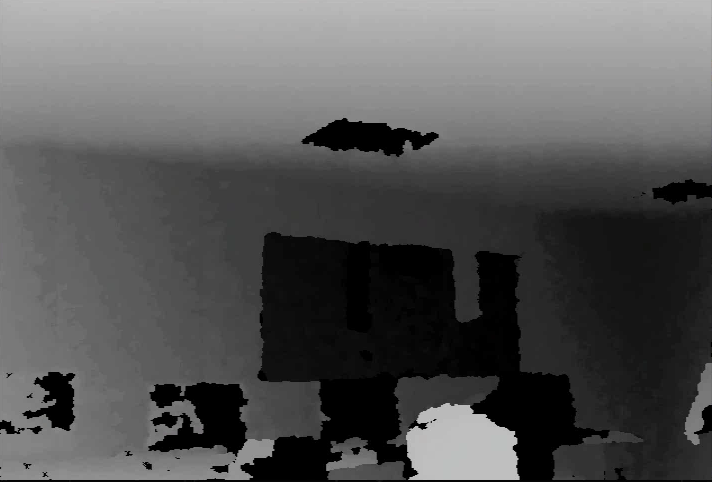
\includegraphics[width=0.24\textwidth]{figuras/5.Testes/deteccao/2.png}}
					\subfloat[] {
						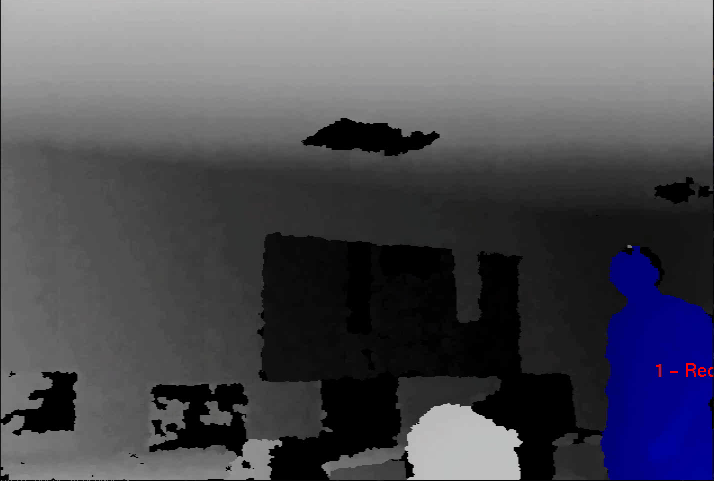
\includegraphics[width=0.24\textwidth]{figuras/5.Testes/deteccao/3.png}}
					\subfloat[] {
						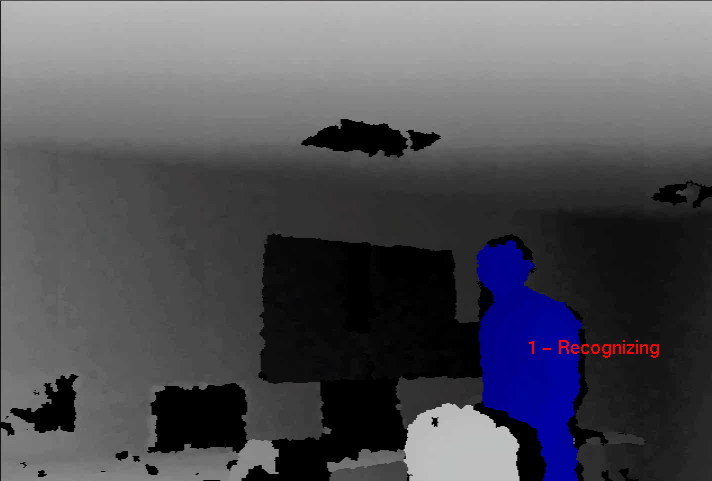
\includegraphics[width=0.24\textwidth]{figuras/5.Testes/deteccao/4.png}}
				\end{center}
				\caption{Momento em que um novo usuário foi detectado pelo Sistema TRUE.}
				\label{fig:testes_deteccao}
			\end{figure}
	    \end{frame}
	    
	    \begin{frame}
	    	\frametitle{Rastreamento - Oclusão}
	    	
			\begin{figure}[htb]
				\begin{center}
					\subfloat[] {
						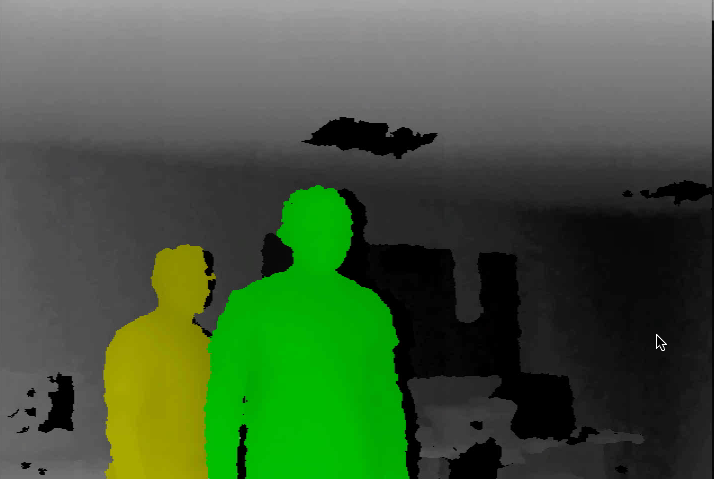
\includegraphics[width=0.19\textwidth]{figuras/5.Testes/oclusao/1.png}}
					\subfloat[] {
						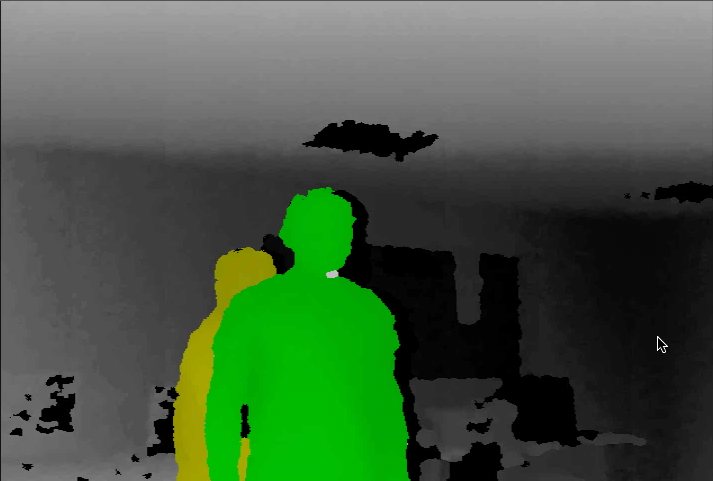
\includegraphics[width=0.19\textwidth]{figuras/5.Testes/oclusao/2.png}}
					\subfloat[] {
						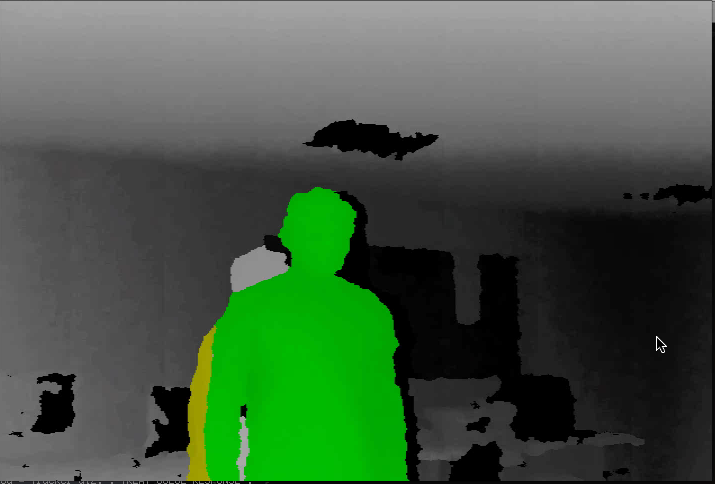
\includegraphics[width=0.19\textwidth]{figuras/5.Testes/oclusao/3.png}}
					\subfloat[] {
						\label{fig:testes_oclusao_ocluso}
						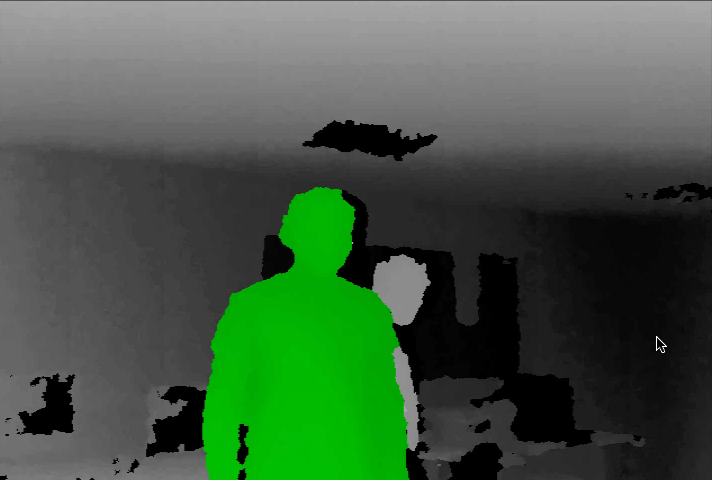
\includegraphics[width=0.19\textwidth]{figuras/5.Testes/oclusao/4.png}}
					\subfloat[] {
						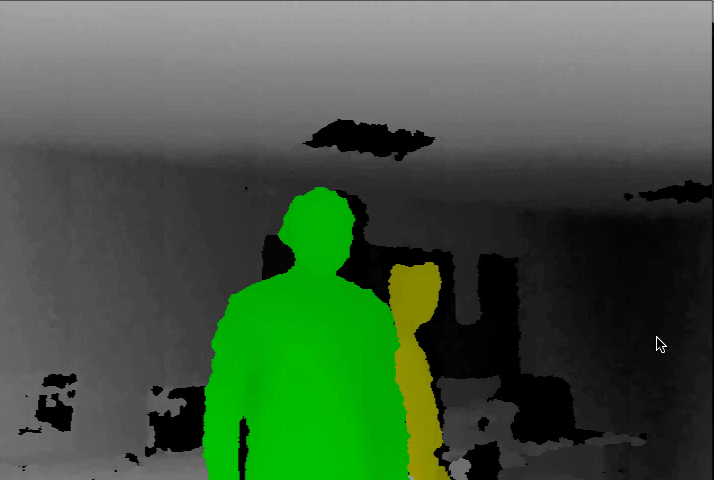
\includegraphics[width=0.19\textwidth]{figuras/5.Testes/oclusao/5.png}}
				\end{center}
				\caption{Oclusão de usuários.}
				\label{fig:testes_oclusao}
			\end{figure}
	    \end{frame}
	    
	    \begin{frame}
	    	\frametitle{Rastreamento - Interferência}
	    	
			\begin{figure}[htb]
				\begin{center}
					\subfloat[] {
						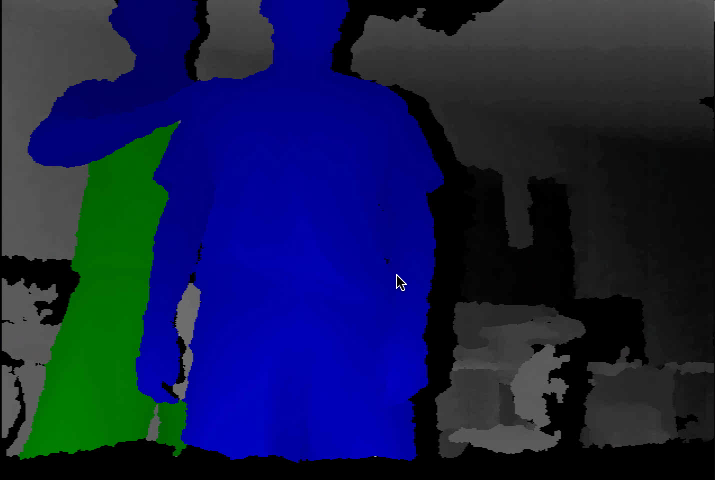
\includegraphics[width=0.32\textwidth]{figuras/5.Testes/relacionamento_com_pessoas/1.png}}
					\subfloat[] {
						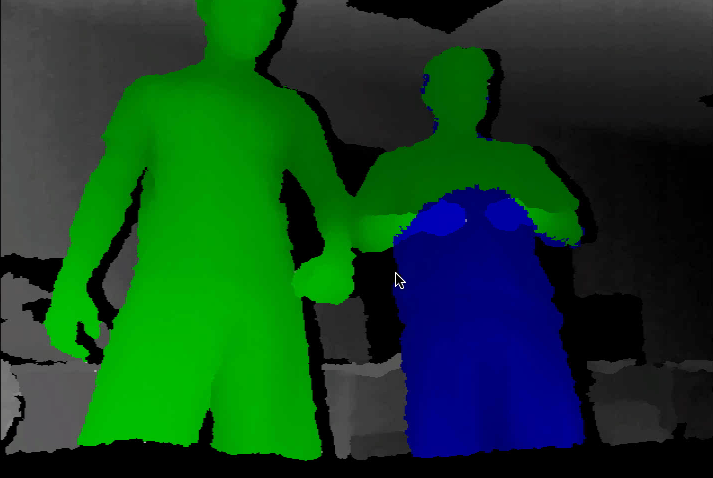
\includegraphics[width=0.32\textwidth]{figuras/5.Testes/relacionamento_com_pessoas/2.png}}
					\subfloat[] {
						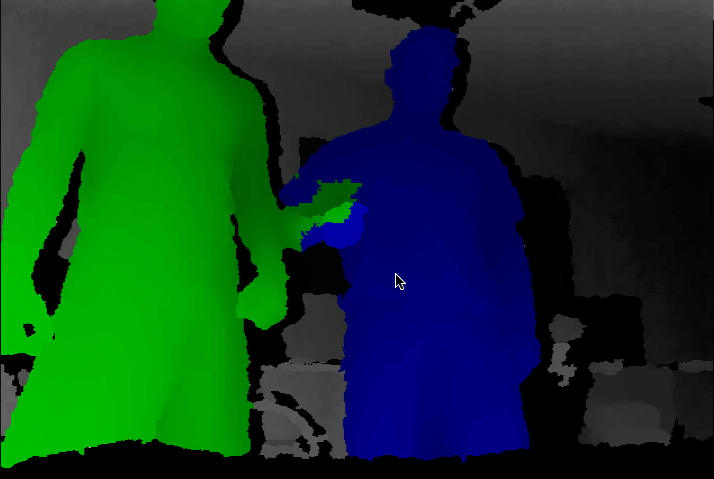
\includegraphics[width=0.32\textwidth]{figuras/5.Testes/relacionamento_com_pessoas/3.png}}
				\end{center}
				\caption{Usuários sofrendo interferência dos que estão ao seu redor.}
				\label{fig:testes_relacionamento_com_usuarios}
			\end{figure}
	    \end{frame}
		
		\begin{frame}
	    	\frametitle{Rastreamento}
			
			\begin{figure}[htb]
				\begin{center}
					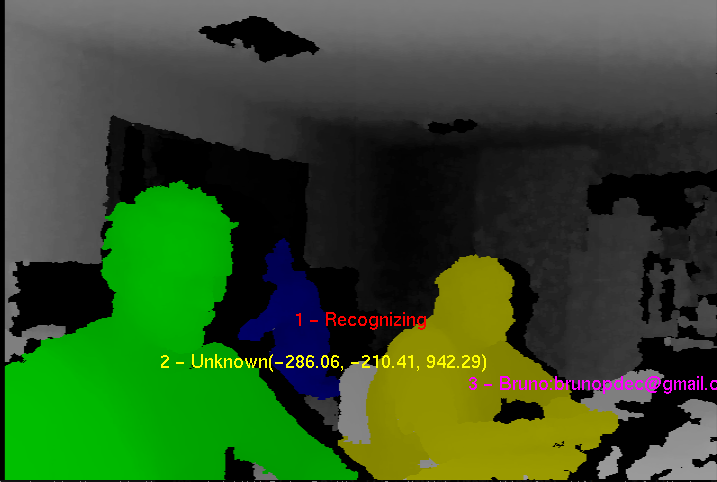
\includegraphics[width=0.9\textwidth]{figuras/5.Testes/oclusao/usuarios-rastreados.png}
				\end{center}
				\caption{Usuários rastreados pelo Sistema TRUE.}
				\label{fig:varios-usuarios-ambiente}
			\end{figure}
	    \end{frame}    
   
   
	% ------------- Resultados obtidos -> Localização -------------
    \subsection{Localização}
    
    	\begin{frame}
	    	\frametitle{Localização - eixo z}
	    	
	    	\begin{figure}[htb]
				\begin{center}
					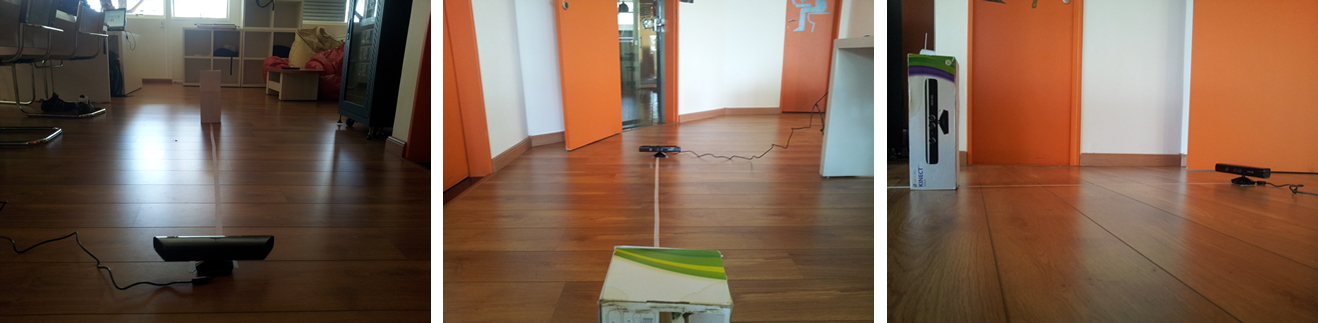
\includegraphics[width=0.95\textwidth]{figuras/5.Testes/teste-eixoz.png}
				\end{center}
			\end{figure}
	    \end{frame}
	    
    	\begin{frame}
	    	\frametitle{Localização - eixo z}
	    	
	    	\begin{figure}[htb]
				\begin{center}
					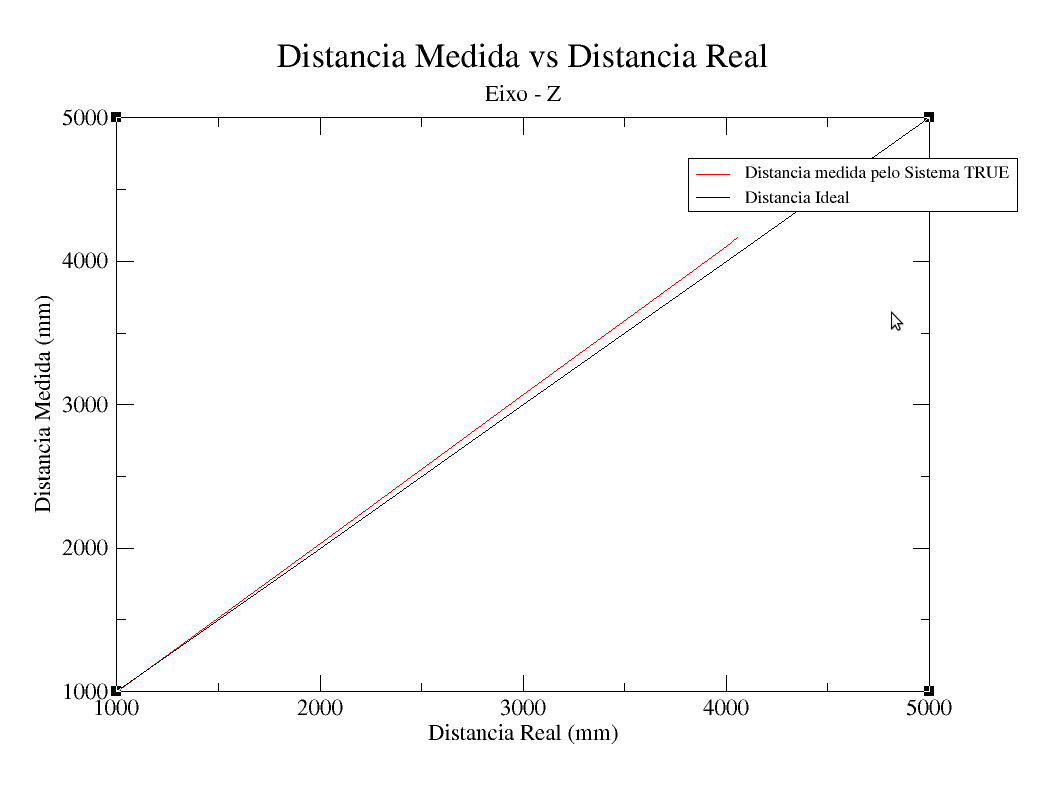
\includegraphics[width=0.95\textwidth]{figuras/5.Testes/grafico-eixo-z.png}
				\end{center}
			\end{figure}
	    \end{frame}
	        
    	\begin{frame}
	    	\frametitle{Localização - eixo x}
	    	
	    	\begin{figure}[htb]
				\begin{center}
					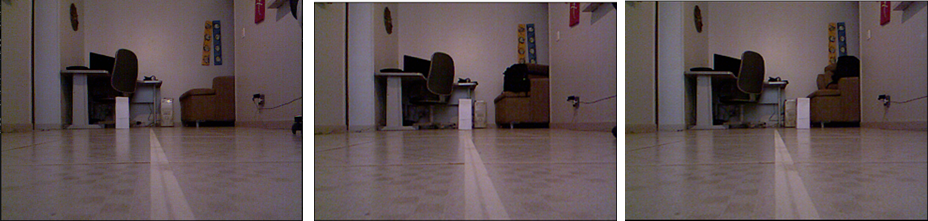
\includegraphics[width=0.95\textwidth]{figuras/5.Testes/teste-eixox.png}
				\end{center}
			\end{figure}
	    \end{frame}
	        
    	\begin{frame}
	    	\frametitle{Localização - eixo x}
	    	
	    	\begin{figure}[htb]
				\begin{center}
					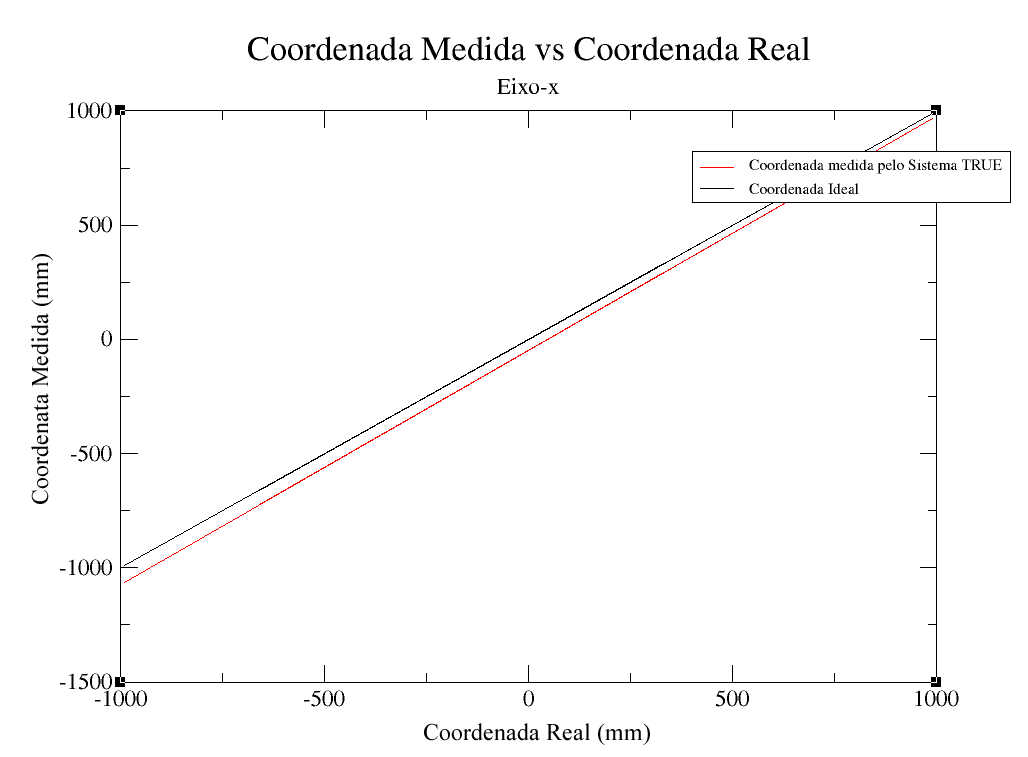
\includegraphics[width=0.95\textwidth]{figuras/5.Testes/grafico-eixo-x.png}
				\end{center}
			\end{figure}
	    \end{frame}
	    
   
	% ------------- Resultados obtidos -> Identificação -------------
    \subsection{Identificação}
	    \begin{frame}
	    	\frametitle{Identificação}
	    	
	    	Primeiro teste
	    \end{frame}
	    
	    \begin{frame}
	    	\frametitle{Identificação}
	    	
	    	Segundo teste
	    \end{frame}
	    
	% ------------- Resultados obtidos -> Integração -------------
    \subsection{Integração}
	    \begin{frame}
	    	\frametitle{Integração}
	    	
	    	\begin{figure}[htb]
				\begin{center}
					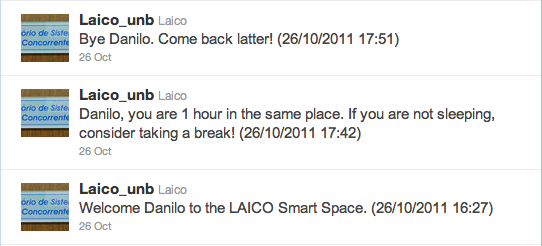
\includegraphics[width=0.95\textwidth]{figuras/5.Testes/tweets.png}
				\end{center}
			\end{figure}
	    \end{frame}
	    
% ------------- Conclusão -------------
\section{Conclusão}

	\begin{frame}
		\frametitle{Conclusão}
	\end{frame}
	
\nocite{fabriciobuzzeto,weiser2,saocarlos,yang,hewitt,violajones}

% ------------- Referências -------------
\section{Referências}

\frame[allowframebreaks]{
  \frametitle{Referências}
  \bibliographystyle{plain}
  \bibliography{bibliografia}
}

\begin{frame}
    \frametitle{ }
    \centerline{Obrigado!}
\end{frame}

\end{document}